\subsection{Constraints on the parameter space due the extended limits}

Taking into consideration these collider limits and also adding the projections of the Direct Detection XENON1T experiment,
we are able to impose the complete set of constraints on the i2HDM parameter space. 
It is worth stressing that as,  before, we  present the limits using  the re-scaled DD cross section 
$\hat{\sigma}_{SI}= R_\Omega\times \sigma_{SI}$, where $R_\Omega = \Omega_{\rm DM}/\Omega^{\rm Planck}_{\rm DM}$, which allows us to take into account additional sources that could contribute to the DM relic density. 

\begin{figure}[htb]
\vskip -0.5cm
\subfigure[Coloured points - always allowed points (AA)]%
{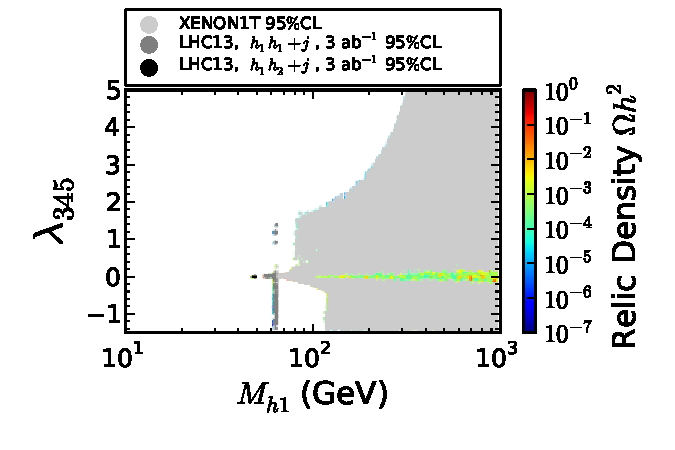
\includegraphics[trim={0 0.5cm 0 0},clip,width=0.49\textwidth]{Figures/Mh1_ld345_Omega_large-coll_a1.pdf}}%
\subfigure[Zoomed  AA region]%
{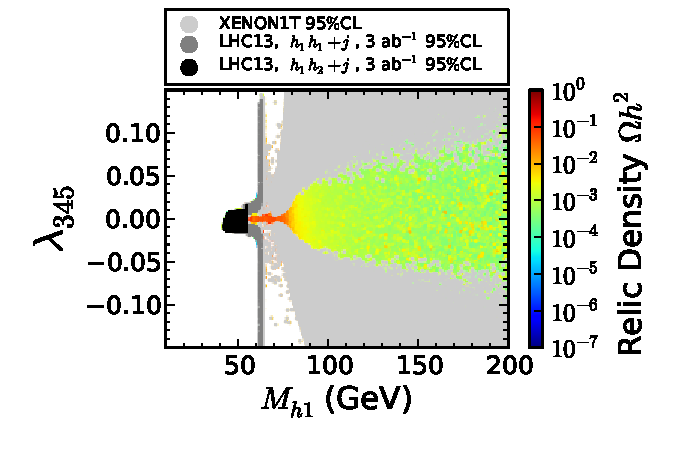
\includegraphics[trim={0 0.5cm 0 0},clip,width=0.49\textwidth]{Figures/Mh1_ld345_Omega_small-coll_zoom_a1.pdf}}\\
\subfigure[Zoomed AA region only for XENON1T constraints]%
{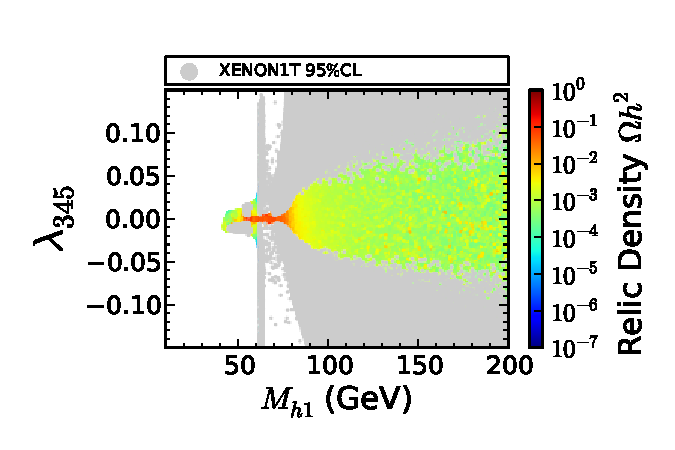
\includegraphics[trim={0 0.5cm 0 0},clip,width=0.49\textwidth]{Figures/Mh1_ld345_Omega_small-coll_zoom_b3.pdf}}%
\subfigure[Zoomed AA region only for the LHC13 constraints from $h1h1+j$ signature]%
{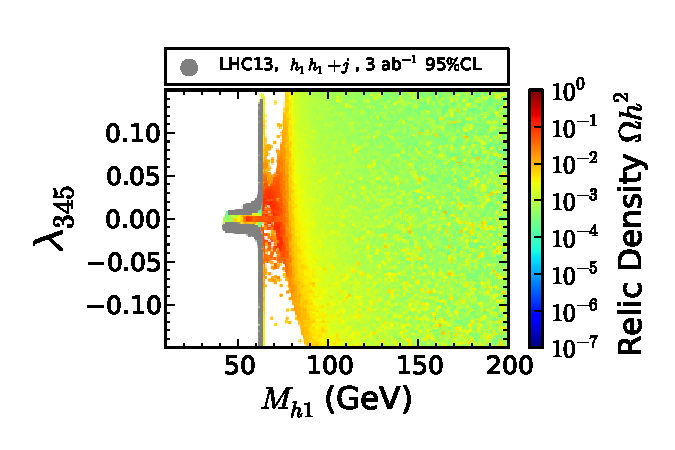
\includegraphics[trim={0 0.5cm 0 0},clip,width=0.49\textwidth]{Figures/Mh1_ld345_Omega_small-coll_zoom_c3.pdf}}
\vskip -0.3cm
\caption{Projection of the 5D random scan of the i2HDM into ($M_{h_1},\lambda_{345}$)
plane and the expected  reach of the LHC@13TeV with 3$ab^{-1}$ of integrated luminosity 
using  $h_1 h_2 j$  and  $h_1 h_1 j$ channels as well as for XENON1T experiment
indicated by black,
dark grey and light grey colours respectively.
Excluded points are plotted on the top of the allowed points   demonstrating the coloured region of the parameter space which will be always allowed (AA):
(a) and (b)
present AA parameter space for the combined constraints for 
large and zoomed ($M_{h_1},\lambda_{345}$) regions respectively;
(c) and (d)
present AA regions for separate  XENON1T and $h_1h_1+jet$ LHC13 constraints
respectively.
\label{collider-XENON1T-constraint}} 
\end{figure}
%
The results of the constraints are presented in Fig.~\ref{collider-XENON1T-constraint} as the color map of DM relic density
in the ($M_{h_1},\lambda_{345}$)  plane together with the projected sensitivity of the LHC@13TeV with 3 ab$^{-1}$ of integrated luminosity 
using  $h_1 h_2 j$  and  $h_1 h_1 j$ channels, as well as a projection for the XENON1T experiment
95\%CL exclusion regions. These constraints are indicated by black, dark grey and light grey colours, respectively.
In this figure we plot {\it excluded points on the top of the allowed points}   demonstrating the coloured region of the parameter space which will be always allowed (AA).
Fig.~\ref{collider-XENON1T-constraint}(a) and Fig.~\ref{collider-XENON1T-constraint}(b)
present AA parameter space for the combined constraints (black on the top of dark grey and dark grey on the top of light grey) for 
large and zoomed ($M_{h_1},\lambda_{345}$) regions respectively,
while  Fig.~\ref{collider-XENON1T-constraint}(c) and  Fig.~\ref{collider-XENON1T-constraint}(d)
present AA regions for separate  XENON1T and $h_1h_1+jet$ LHC13 constraints
respectively. From Fig.\ref{collider-XENON1T-constraint}a-c 
one can see how constraints from the LHC and XENON1T are complementary to each other.
One can see that XENON1T will exclude large $M_{h_1}$ masses
for large enough values of  $\lambda_{345}$ while the LHC will probe the region of smaller values of  $\lambda_{345}$ for $M_{h_1}$ below the $M_H/2$ threshold using the
$h_1h_1j$ channel, and will cover all values of $\lambda_{345}$
using the $h_1h_2j$ channel for  $M_{h_1}$ below 55 GeV.

Besides the AA region it is informative to find and analyse the region
with {\it allowed points on the top of excluded points}, therefore the
black and grey colours
present the region which will be always excluded (AE)
or probed by the above experiments. Such region is presented 
in Fig.~\ref{collider-XENON1T-constraint-AE}(a,b)
in exact analogy to  Fig.~\ref{collider-XENON1T-constraint}(a,b).
%
\begin{figure}[htb]
\vskip -0.5cm
\subfigure[Grey-black points - always excluded points (AE)]%
{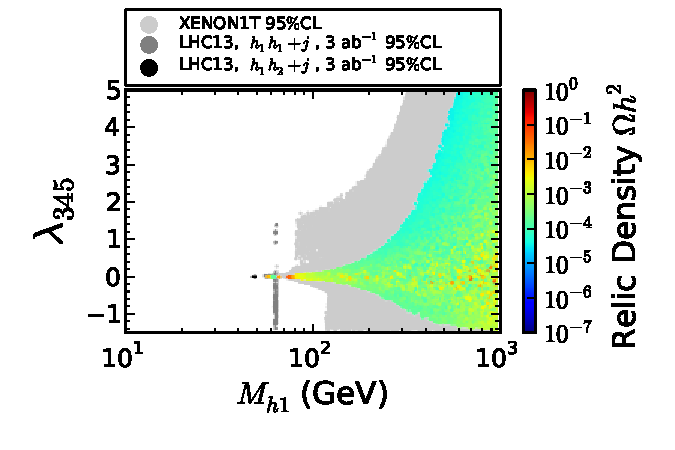
\includegraphics[trim={0 0.5cm 0 0},clip,width=0.49\textwidth]{Figures/Mh1_ld345_Omega_large-coll_a2.pdf}}%
\subfigure[Zoomed region with AE points]%
{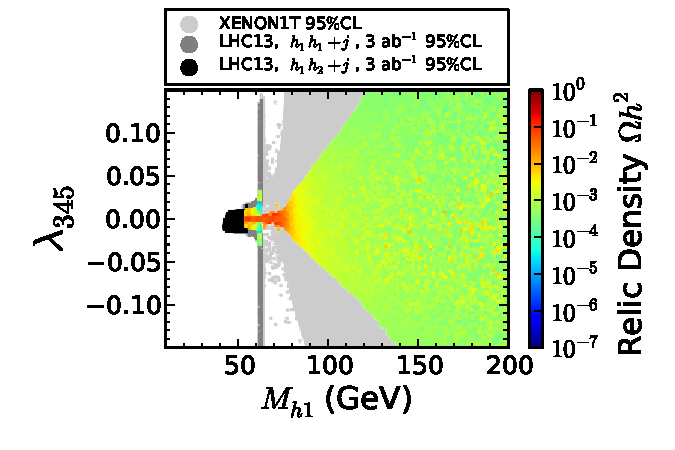
\includegraphics[trim={0 0.5cm 0 0},clip,width=0.49\textwidth]{Figures/Mh1_ld345_Omega_small-coll_zoom_a2.pdf}}
\vskip -0.3cm
\caption{Projection of the 5D random scan of the i2HDM into ($M_{h_1},\lambda_{345}$)
plane and the expected  reach of the LHC@13TeV with 3$ab^{-1}$ of integrated luminosity 
using  $h_1 h_2 j$  and  $h_1 h_1 j$ channels as well as for XENON1T experiment.
Allowed points are on the top of the excluded ones, therefore
the black and grey colours
present  the region which will be always excluded (AE)
or probed by the above experiments.
\label{collider-XENON1T-constraint-AE}} 
\end{figure}

When comparing Fig.~\ref{collider-XENON1T-constraint}(a,b) and Fig.\ref{collider-XENON1T-constraint-AE}a,b 
--- i.e. the plots with AA versus AE points, --- one observes
a big difference between the order of the overlay of the excluded and allowed points.
This is related to the fact that the $\Omega_{\rm DM} h^2$ can substantially vary:
even for  fixed $M_{h_1}$ and  $\lambda_{345}$ values,
a large $M_{h^+}$ or $M_{h_2}$  can provide respectively large quartic couplings $h_1 h_1 W_L W_L$ and  $h_1 h_1 Z_L Z_L$, see Eq.~(\ref{tildelam345}), 
which lead in their turn to an effective $h_1 h_1 \to VV$  annihilation. This brings the relic density down and 
avoids the XENON1T constraints (once we use DD rates re-scaled to relic density).
In the ($\lambda_{345},M_{h_1}$) plane, for example, these points overlap with the points 
where the quartic couplings mentioned above are small and the  $\Omega_{\rm DM} h^2$ (and respectively exclusion) is driven only by $\lambda_{345}$. 
So the most complete picture comes from the combination of AA and AE plots:
the most conservative allowed region comes from AA plots of Fig.~\ref{collider-XENON1T-constraint}, while the most conservative exclusion region
is presented by AE plots of Fig.\ref{collider-XENON1T-constraint-AE}.

%
\begin{figure}[htb]
\subfigure[]{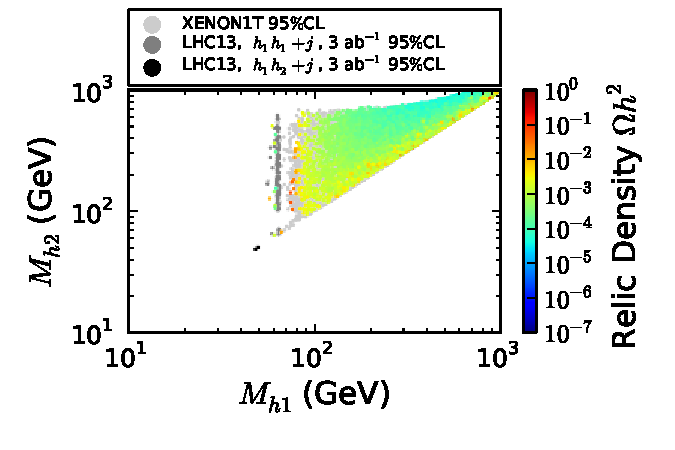
\includegraphics[trim={0 0.5cm 0 0},clip,width=0.5\textwidth]{Figures/Mh1_Mh2_Omega_large-coll_a2.pdf}}%
\subfigure[]{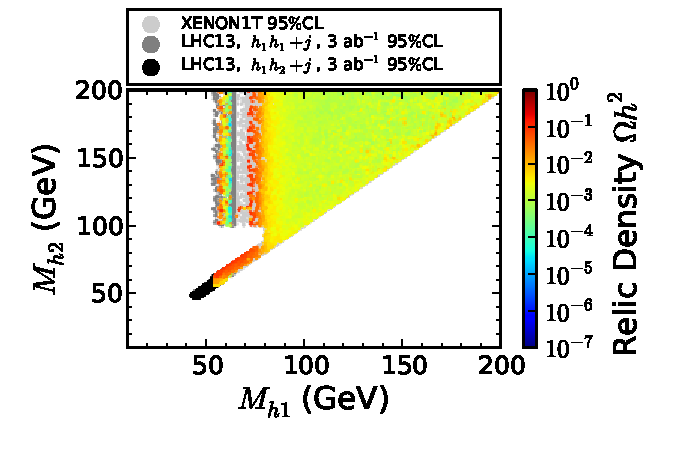
\includegraphics[trim={0 0.5cm 0 0},clip,width=0.5\textwidth]{Figures/Mh1_Mh2_Omega_small-coll_a2.pdf}}\\
\subfigure[]{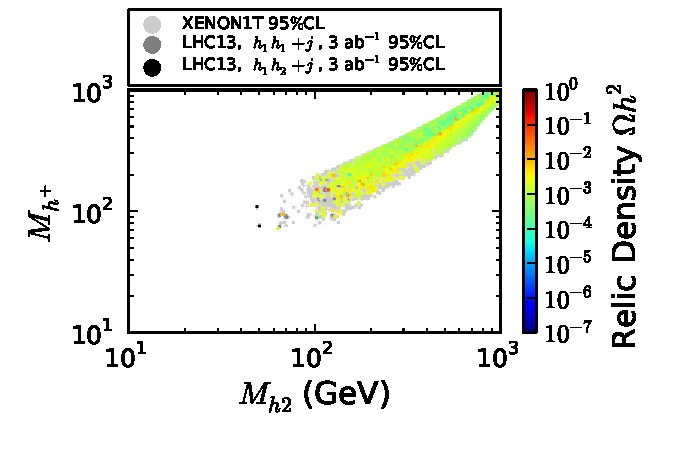
\includegraphics[trim={0 0.5cm 0 0},clip,width=0.5\textwidth]{Figures/Mhc_Mh2_Omega_large-coll_a2.pdf}}%
\subfigure[]{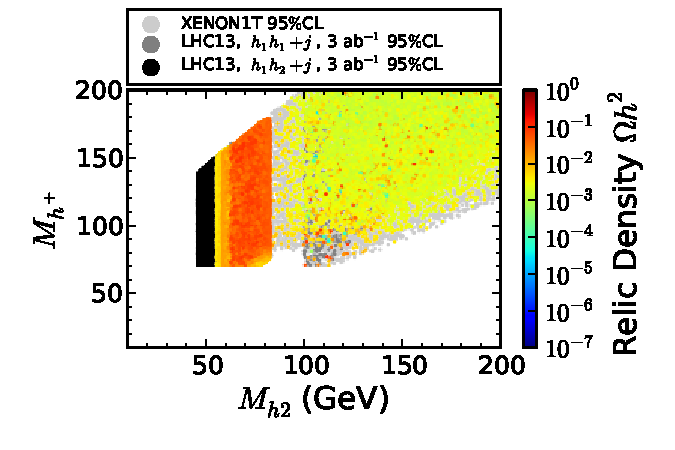
\includegraphics[trim={0 0.5cm 0 0},clip,width=0.5\textwidth]{Figures/Mhc_Mh2_Omega_small-coll_a2.pdf}}\\
\caption{\label{collider-XENON1T-constraint-AE-other}
Projection of the 5D random scan of the i2HDM into ($M_{h_1},M_{h_2}$) (a,b)
and ($M_{h_2},M_{h^+}$) (c,d) planes
and the expected  reach of the LHC@13TeV with 3$ab^{-1}$ of integrated luminosity 
using  $h_1 h_2 j$  and  $h_1 h_1 j$ channels as well as for XENON1T experiment.
Allowed points are on the top of the excluded ones,
presenting AE points. The left panels (a,c) present a bigger region of the parameter space, while the
right ones (b,d) present a zoomed region with AE points.} 
\end{figure}
%
From Figs.\ref{collider-XENON1T-constraint} and \ref{collider-XENON1T-constraint-AE}
one can see  that imposition of the XENON1T constraint reduces substantially the parameter space, greatly expanding the previous limits imposed by LUX. This effect is not so evident in the other planes, presented in Fig.\ref{collider-XENON1T-constraint-AE-other}
in analogy to Fig.\ref{collider-XENON1T-constraint-AE},
because the spin-independent cross section $\hat{\sigma}_{SI}$ for DD is driven by the $t$-channel Higgs boson exchange 
and therefore is proportional to $\lambda_{345}^2$.
\begin{figure}[htb]
\subfigure[]{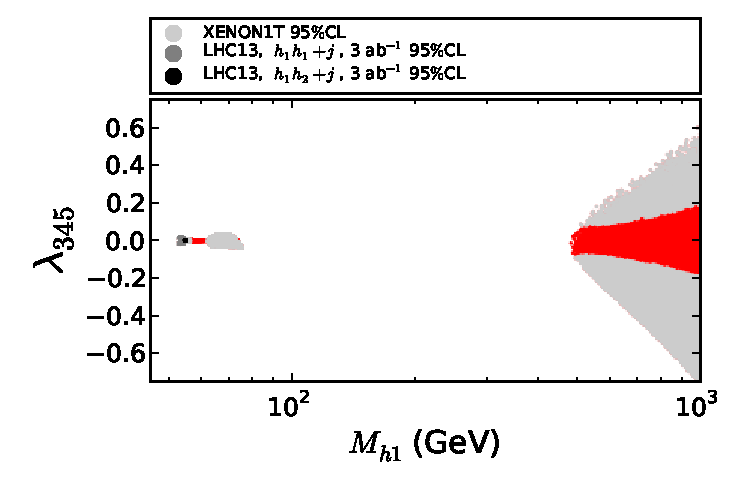
\includegraphics[trim={0 0.5cm 0 0},clip,width=0.5\textwidth]{./Figures/Mh1_ld345_Omega_relic-large-coll_zz-large-monoc.pdf}}%
\subfigure[]{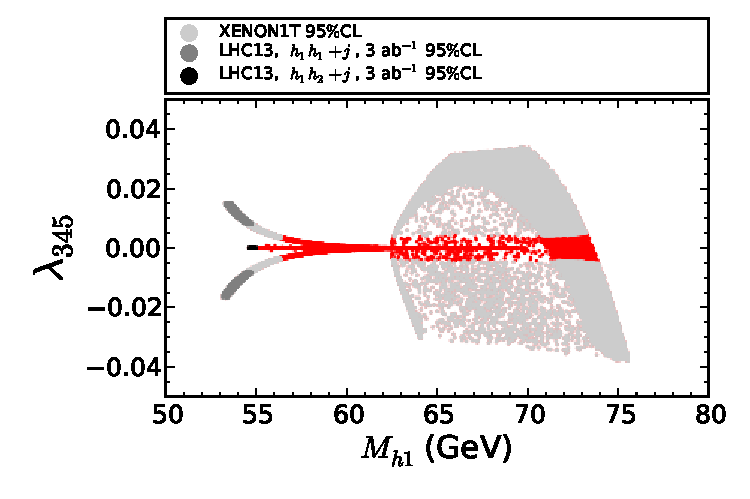
\includegraphics[trim={0 0.5cm 0 0},clip,width=0.5\textwidth]{./Figures/Mh1_ld345_Omega_relic-small-coll_zz-monoc.pdf}}\\
\subfigure[]{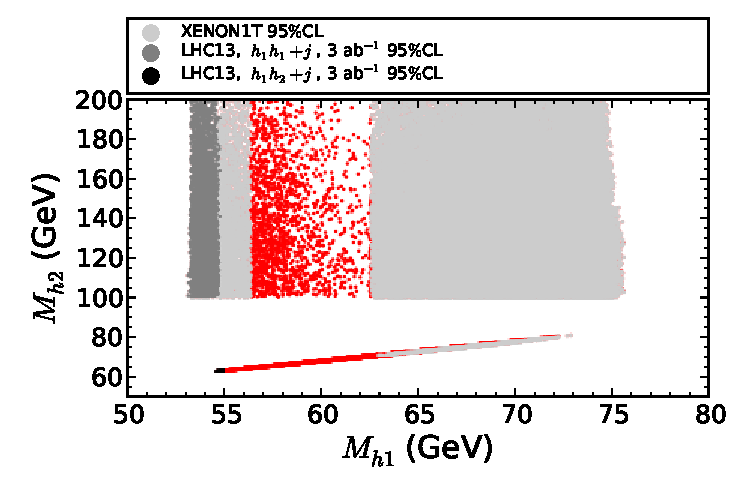
\includegraphics[trim={0 0.5cm 0 0},clip,width=0.5\textwidth]{./Figures/Mh1_Mh2_Omega_relic-small-coll_zz-monoc.pdf}}%
\subfigure[]{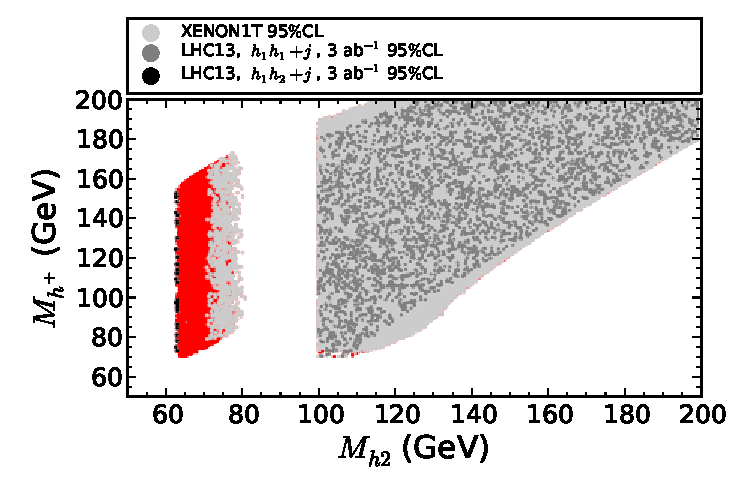
\includegraphics[trim={0 0.5cm 0 0},clip,width=0.5\textwidth]{./Figures/Mhc_Mh2_Omega_relic-small-coll_zz-monoc.pdf}}
\caption{2D projections of the 5D random scan of the i2HDM satisfying all constraints (Cut-1 to Cut-4) considered above for Fig.(\ref{fig:dm-i2hdm},\ref{fig:dm-i2hdm-small}) plus the lower limit on the constraint on relic density given by Eq.(\ref{eq:planck-limit}), taking in consideration the collider limits of mono-jet signatures at 13 TeV with 3$ab^{-1}$ of integrated luminosity and the projections of the DD XENON1T experiment. In the first row we present the parameter space of the plane ($M_{h_1},\lambda_{345}$) in the range $\subset $[10~GeV--1000~GeV]). In the second row we present the planes ($M_{h_1},\lambda_{345}$) and ($M_{h_1},M_{h_2}$) in the range $ \subset $[50~GeV--80~GeV]).} \label{fig:dm-i2hdm-LHC-DD}
\end{figure}

One should also stress again the  importance of the   $pp \to h_1h_2+j$ process,
using which  one can exclude $M_{h_1}<55$ GeV when  $M_{h_2}-M_{h_1}$ is small
for all values of $\lambda_{345}$.
 This is shown clearly  with the black dots in the Fig.~\ref{collider-XENON1T-constraint-AE-other}(b,d) where the (co)annihilation and respective mass degeneracy between $M_{h_1}$ and $M_{h_2}$ take place. Finally the $pp \to h_1 h_1 + j$ process imposes an extra constraint for the zone with low relic density corresponding to the $h_1h_1 \to H$ resonant annihilation just above $M_{h_1}=M_H/2$. In this case the invisible Higgs decay $H \to h_1h_1$ is closed and there is no restriction on $|\lambda_{345}|$, as we can see in Fig.~\ref{collider-XENON1T-constraint-AE-other}(b,d) represented by the dark grey points.

We have also found the  projected limits from colliders of mono-jet signatures  and the XENON1T DD experiment for the i2HDM points which satisfy both the upper and lower PLANCK limits, Eq.(\ref{eq:planck-limit}). In this case, the scattering cross section $\sigma_{SI}$ is not re-scaled, because we are in the zone with the right amount of DM relic density. The results of these constraints are presented in Fig.~\ref{fig:dm-i2hdm-LHC-DD} as a scatter plot where the red zones represent the right amount of DM relic density. In the first row we show the parameter space of the plane ($M_{h_1},\lambda_{345}$) in the full
mass range from 10 to 1000~GeV. In the second row we present the planes ($M_{h_1},\lambda_{345}$) and ($M_{h_1},M_{h_2}$) but in a narrow mass range 
between 50 and 80~GeV.
%

As we can see, the incorporation of the DD constraint sets important restrictions on the parameter space. Still, in Fig.~\ref{fig:dm-i2hdm-LHC-DD}(a) there is a zone in the upper mass range that is not ruled out. Also in the low mass range there is a region between 55 GeV $< M_{h_1} <$ 74 GeV
which survives the restrictive constraint for small values of $\lambda_{345}$. We zoom into the surviving low mass region in Figs.~(\ref{fig:dm-i2hdm-LHC-DD}(b,c). Because of the improved limits of the DD experiment, the parameter $\lambda_{345}$ is very sensitive to scattering cross section, 
which sets a limit of $|\lambda_{345}|<0.01$ for this mass range.

The $pp \to h_1h_2+j$ process sets the exclusion limit for $M_{h_1}<55$ GeV (black dots) at the beginning of the $h_1 h_2$ coannihilation region represented by the thin horizontal strip for very small values of $\lambda_{345}$ in Fig.~\ref{fig:dm-i2hdm-LHC-DD}(b), which is also seen in the lower part of Fig.~\ref{fig:dm-i2hdm-LHC-DD}(c). The $pp \to h_1 h_1 + j$ process imposes an extra constraint on the lower mass zone where the DM annihilates through Higgs boson exchange and is visible in Fig.~\ref{fig:dm-i2hdm-LHC-DD}(b) in the shape of two symmetric wings for negative and positive values of $\lambda_{345}$. This excludes the $M_{h_1}<55$ GeV region. XENON1T will improve this constraint and exclude the $M_{h_1}<56.5$ GeV region.